%!TEX root = main.tex

%===============================================================================
%     File: ch_machine_learning.tex
%    Author: Juan de Monasterio
%    Created: 08 Feb 2017
%  Description: Chapter : Machine Learning
%===============================================================================

\chapter{Machine Learning}\label{ch:machineLearning}

This chapter will present an elementary introduction to the theory behind Machine Learning.
The concepts and ideas developed here will be exemplified on concrete applications of the processed CDR data, using a Logistic Regression classifier.
Also, the chapter will formulate the tasks that will be solved in later chapters, as means of transforming the long-term human migrations into a supervised classification problem.

Most of the discussions here are based on information extracted from two distinguished textbooks: \citep{bishop-patternRecognition} and \citep{hastie-elemstatslearn}.
Some fundamental concepts and material were also referrenced from\citep{scikit-learn}.
When other texts were used, they have been cited correspondingly in the text, and, where not specified, the reader can assume that the proof is based from the textbooks above mentioned.

\section{Overview of Supervised Classification Applications}\label{section-supervised-learning}


Machine Learning is divided into two main categories: Supervised and Unsupervised Learning.
If we consider $Y \in \mathbb{R}^n$ be the output vector of the model and $X \in \mathbb{R}^{n \times p}$ be the input matrix: supervised learning algorithms produce outputs from input data i.e.\ for each instance $x \in X$, the computer has access to examples of outputs and tries to reproduce them based on information contained in $X$.
In this context, the algorithm is generally referred to as a \textit{learner}.

The second class of problems is where there is no output $Y$ in the data.
In this scenario the most common objectives are clustering samples, density estimation and data compression.
A linear regression and K-means clustering are examples of algorithms in both categories respectively.

In supervised learning, tasks are sub-categorized by the nature of the problem.
If the type of the output variable $Y$ takes a (generally \textit{small}) discrete set of values, then it is said that it is a supervised \textit{classification} problem.
On the other hand, when the output takes continuous (or dense in an open set of $\mathbb{R}$) range of \textit{quantitative} values, it is said to be supervised \textit{regression} problem.
Note that regression problems can be encoded into classification problems by grouping the output values into categories in which each takes a range of output values.

Suppose now that  aim is to predict $y$ given a new sample $x$.
We would have that for supervised regression problems, $y$ will comprise a continuous variable.
On the other hand for classification problems $y$ will represent a label for a certain class.
For the case of $K$ classes, we can say that $y$ takes values in the ranges $0$ through $K-1$ or $1$ through $K$.
In both cases, the joint probability distribution $p(X, Y)$, called the \textit{true} distribution, gives all the information we need on these two variables.
Yet the characterization of this probability is most often unknown.

Noting this, the idea is to use estimations and predictions on the \textit{most likely} values for new samples and take decisions based on past information.
These decisions will be based on the most probabilistic characterization of the problem, from the data we have.
For this work we will focus on the classification aspect of machine learning.

We also note that when dealing with these problems, the theoretical and the computational aspects are both of interest.
It is reasonable to say that the data, taken as an input to the problem, limits the available solutions and the same goes for the algorithms used in the solution process.
These need to take into consideration aspects such as the software and hardware available, as well as time or resource constraints imposed by the problem itself.
As such, these are expected to be executed in a reasonable amount of time, required by the task's specification, and limited by the computing power available.\footnote{Here the word \textit{reasonable} is used in a broad sense.
It will depend entirely on time constraints, computational capacity, usage and other aspects of each learning application.} There can be problems which require that the algorithm output predictions in \textit{real-time}, to the resolution of milliseconds.

For example, if we picture a system where credit-card transactions need to be approved or labeled as a fraud, we would expect the system needs to quickly respond if the transaction is approved or not.
Other use cases might require the system to process a big volume of data at once, not a single event, but a batch of these and produce and output answer.
The production system needs to be prepared to run \textit{lean} with a big inflow of data, without exceeding the hardware capacity.

These examples show that for a given problem, there are multiple algorithms available for use, but while all of them are theoretically doing the same task, we must also consider the practical advantages of them.
Computational efficiency and \textit{scalability} are relevant when working in these kind of problems.
Even though we won't delve into these aspects in this work, it has an important consideration in Machine Learning applications.
And these also influence the way research is conducted in this area.


In its essence, a machine learning method is a probabilistic model built from data and in this way it is very similar to a statistical model.
However, it differs specially in that its focus is generally on the models' predictive abilities more than in the model's parameters estimates~\citep{breiman-statisticalmodeling}.
The algorithms will be built and used for a given phenomena, to try and replicate it as best as possible without really identifying the true nature of the mechanisms behind this phenomena.
As such, most applications will try to \textit{imitate} the task's behavior rather than try to identify the real system behind it.
%on this matter It also puts a great amount of weight on efficiency and computational scalability.

%At this point it is important to start noting

These subtle differences in the machine learning approach of a problem is also reflected in the terminology used by the field.
For the methods introduced here, we know that other disciplines often speak about them in different terms and this difference is certainly notable with classic statistics.

Where we can, we will be identifying these differences along the text.
As a start, the \textit{dependent} $Y$ is called the target or label and the \textit{independent} variables, \textit{covariates} or \textit{input variables} are named \textit{features} in this case.
%Labels that are representing categorical or discrete variables are also named factors or \textit{qualitative} variables.

\section{Long-term Human Migrations Classification}\label{long_term}

Starting from the two-year CDR dataset we have described in \cref{ch:descr-risk}, we introduce our set of tasks defined to find how to tackle the long-term human migrations problem under a supervised classification framework.
This is convenient to do so given the nature of our problem.

We intend to develop a set of machine learning methods that will aid us in further characterize and analyze the mobility of users between regions.
These will help us establish to what extent the CDRs allow us to predict a user's past home and migration movement across both endemic and non-endemic regions.
More precisely, we would like to explore the relationship of the dataset attributes based on calling patterns across regions to the movement of humans.
Where possible, we would like to establish which features are most relevant for our predictors.
% In an ideal case, we would like to have a certain insight into the causes of these movements, without being able to make any causal inferences.

To start off, we need to introduce some notation to describe different sets of users.
For this, we will divide them into distinct sets, marked by their behavior across each time period:

\begin{definition}\label{def:endemic_sets_periods}
	(i) $EU_{1}$ are the users that lived in the endemic region in period $T_1$ while $EU_{0}$ are the users that lived in the past (period $T_0$);
	(ii) their set complements are defined as ${ EU_1 }^{\complement}$ and ${ EU_0 }^{\complement}$ respectively and
	(iii) the user's home antenna in each period will be referred to as $H0_u$ and $H1_u$, following the same time convention as before.
\end{definition}


%We will have these can be differentiated for both periods by

Keeping the above in mind, we divide our task into four problems.
These will serve as different perspectives of the mobility issue and all of them together will give us a principled understanding of the problem.

It is important to note that all problems are solved with user data extracted from their communications during $T_1$.
This means that no information from $T_0$ will be used as input to the statistical models.

We process the raw data to build our target variable which will be determined as $Y$ and it will be defined for every user $u$.
Then the only difference among all of the problems will be in how the target variable is defined\footnote{In reality, certain variations of the data were considered too, where best performing features were filtered from the dataset to explore how this decreased the overall prediction ability of the algorithm.}.


We present here the list of problems that will be used throughoutthis work:


\begin{problem}\label{target1}
We want to infer which users lived in the endemic region in the past:
		\begin{align*}
		Y_u =
		\begin{cases}
		&1 \ \mbox{if} \ u \in EU_{0} \\
		&0 \ \mbox{if not}.
		\end{cases}
		\end{align*}
\end{problem}

With this definition and using the description of the features extracted from the data in \cref{ch:descr-risk}, we observe that here the information of a user's endemicity $EU_{1}$ is used to predict their membership to $EU_{0}$.
And it would not be of much surprise to know that these two variables are indeed highly correlated with a value of 93\%.
This means that, overall, the feature is a good predictor of the target variable causing algorithms to be heavily weighted towards this attribute.
We could use this single feature as a basic algorithm to build a simple predictor.

To prevent this from happening and to capture the change in endemicity for a small groups of users, we decided then to hide this feature when solving \cref{target1}.

% Other features, such as the number of calls to endemic regions, are correlated to the target variable. This is an expected behavior since most people use cellphones for local calls only. Let these correlations are not as high as with the $EU_{1}$ variable. Also, given the assumptions used in

% However we have not excluded any other features
% are locally  an and given the assumptions used maps in \cref{}, this is a result which

\begin{problem}\label{target2}
We want to infer which users lived in $E_Z$ in the past and then migrated:
	\begin{align*}
				Y_u =
				\begin{cases}
					&1 \ \mbox{if} \ u \in EU_{0} \cap { EU_{1} }^{\complement}  \\
					&0 \ \mbox{if not}.
				\end{cases}
			\end{align*}
\end{problem}

In this task, we have not excluded any attributes from the data since this problem does not carry the feature-target correlation problems like before.
Recall from \cref{tab:changes} that we have at most 23 thousand users that satisfy this condition over more than a million users.
This strong unbalance in the target class proves to be a much harder problem to solve than in \cref{target1} since these users become harder to find.
If not correctly taken into account, the error over the small class would be dominant of the overall prediction.

It is relevant to note here that we are ignoring any relevant information about the user's endemicity or current state of residence.
Otherwise we would have a perfect correlation between $Y_u=0$ and being currently endemic, or living in an endemic state.

% This is because we could use a dumb predictor to always output the value of the bigger class.


\begin{problem}\label{target3}
Users that migrated between regions.
\begin{align*}
			Y_u =
			\begin{cases}
				&1 \ \mbox{if} \ u \in (EU_{0} \cap { EU_{1} }^{\complement}) \cup (EU_{1} \cap { EU_{0} }^{\complement}) \\
				&0 \ \mbox{if not}.
			\end{cases}
		\end{align*}
\end{problem}

This task has a similar difficulty as in the previous one, yet there are more users satisfying this condition.
The difference relies in that cross-migrations are not as important to our study as migrations directly from the endemic region.
Still, we define this task with hope to eventually find some unexpected insights.


\begin{problem}\label{target4}
Users that migrated from the endemic region, but conditional to users which are currently not endemic.
This means that we will only consider users which $u \in EU_{1}^{\complement}$ as a base set.

\begin{align*}
			Y_u =
			\begin{cases}
				& 1 \ \mbox{if} \ u \in ( EU_{0} \cap { EU_{1} }^{\complement})    \\
				& 0 \ \mbox{if} \ u \in ( { EU_{1} }^{\complement} / EU_{0}).
			\end{cases}
		\end{align*}
\end{problem}

An important observation is that at this point we are looking at a reduced instance of our CDRs, because we are only considering currently non-endemic users other than the whole sample population.
Still, we are observing a total of more than a million users for this case.


% \begin{problem}\label{target5}
% As a \textbf{bonus} problem and for exemplary reasons, we considered tried to detect if a user has a high mobile footprint $M_u$, as defined in \cref{section:def_mobility_diameter}.

% 	\begin{align*}
% 		Y_u =
% 		\begin{cases}
% 			&1 \ \mbox{if} \ {M_u >  1000 } \\
% 			&0 \ \mbox{if not}.
% 		\end{cases}
% 	\end{align*}

% \end{problem}


We can see from what was mentioned before that not all problems can be represented by the same dataset.
The limitations on what is available as our input set $X$ attributes or samples.
For example, we said that in \cref{target1} we have no limitations to use that $u \in EU_{1}$, yet we decide to ignore this highly correlated feature.
By not doing so, we  would be implicitly introducing the target variable as an attribute.
Thus, appropriate care must be taken in each case over which attributes should be taken as inputs for the models.


With \cref{target1,target2,target3,target4}, we continue on to define and illustrate techniques for supervised classification.
Throughout \cref{ch:modelSelection,ch:ensembleMethods,ch:results,ch:conclusions} we will come back to these problems by applying them with the techniques and methods we discuss.


\section{A working example of a Machine Learning setup}\label{section-example}

In our work we take advantage of the volume of samples, where, as explained in \cref{ch:descr-risk}, almost 1.5 million users.
This allows us to randomly split the dataset into training and test sets that do not overlap and which contain 70\% and 30\$ of all samples respectively.
The test set will be a part of the model building process and we will only use it at the end of the process.
No information from the test set should be accessed during the construction of the models.

We will note the training and the test sets by $\mathcal{T}$  and $\mathcal{T_s}$.
Both $\mathcal{T}$ and $\mathcal{T_s}$ will take the form of a paired couple of datasets $(X,Y)$ where $X \in \mathbb{R}^{n \times p}$ and $Y \in \mathbb{R}^n $.


The difference will lie in the way each set is used to computationally build a probabilistic model.
The idea is that the test set will not take part in building the machine learning model and will be used only to evaluate its performance.
In this way it is acting as a simulation of the algorithm's performance, by evaluating over \textit{new} samples.\footnote{
	We make an important remark here that the user's privacy is ensured by not providing a direct identifier of the person.
	All users are distinguished with their \textit{user\_id} which is information given by the TelCo with a salted hash transformation.
	In this way, we are unable to use these identifiers in other data sources other than the specific one used for this work.}
This makes sense knowing that the objective is to build a probabilistic model which has the capacity to correctly predict the output class instances for new data objects, based on having seen information of objects from $\mathcal{T}$.
The samples from $\mathcal{T_s}$ will take on this role.


As an example, let's consider a reduced training dataset built from Call Detail Records (CDRs), where samples are calls being made by users who can belong to any of the following provinces: \textit{Buenos Aires}, \textit{Cordoba} and \textit{Santa Fe}.
%\url{http://stackoverflow.com/}
%\footnote{For more information on this set, a historic review is given at \url{https://en.wikipedia.org/wiki/Iris_flower_data_set}}.
Five measurements were taken on all of the observations to account for the user's number of calls and total minute duration of calls and all data was extracted from a week of logging measurements.
Below we print a short overview of this dataset:

\begin{table}[ht]
\caption{{Head of the raw CDR dataset.
 three-row mock example of calls.}}
\label{tab:sample_CDR}
\centering
\begin{tabular}{ l l l l l l }
\toprule
User & CallsWeekend & TimeWeekend & CallsWeekDays & TimeWeekday & Province \\
\midrule
BA343E & 15 & 89 & 8 & 24 & \textit{Santa Fe}\\
73F169 & 10 & 121 & 2 & 98 & \textit{Cordoba} \\
EA23AD & 12 & 43 & 5 & 154 & \textit{Buenos Aires} \\
\bottomrule
\end{tabular}
\end{table}


In $X$ a row is representing the available data processed for each user, and the columns represent the features which are the different types of measurements or information on that user.
In other settings the features would be known as covariates or independent variables.
%In general, most machine learning problems will be associated with a training set $\mathcal{T}$ of similar form as the one shown before.
It is not uncommon to represent data in with rows as observations or \textit{samples} and columns are measurements or \textit{features} of our samples.

More specifically, the $jth$ column of $X$, or equivalently the $jth$ feature of the dataset, is denoted by $X^j$.
In a similar way, the $ith$ row or sample of $X$, is denoted by $X_i$, or $x$, when it is clear from context or when we are referring to a generic sample.
A similar notation is used with the outputs, where $Y_i$ or $y$ will be used to denote the target of a specific sample, depending on context.

So here, the training set $\mathcal{T}$ is used to algorithmically create a function which maps inputs to outputs,  whilst the test set $\mathcal{T_s}$ will be used to measure how \textit{well} this mapping would behave in real situations, given a way of measuring this performance.

In this particular example, even though the last column of the dataset in \cref{tab:sample_CDR} is not a measurement \textit{per se}, it provides information on each user's province of residence.
With this we can map users to \textit{classes} which conform the partition of the set of provinces.

Hereon, there are various questions one could try to answer using this dataset.
Examples of problems that a machine learning algorithm could tackle could be:
\begin{itemize}
\item Predict a user's province when given information on only the first four features.
\item Predict a user's number of calls made on weekends when given information on the last four features.
\item Give an estimate of the probability density function of user's calls duration, during weekdays.
\end{itemize}

These questions can be shaped into the form of a target variable to define a concrete Machine Learning problem.

The first two of the problems above defined are examples of a supervised learning task.
For each, the $Y$ variables or \textit{labels} are respectively the last and first features (columns in the dataset).
Even more, the first problem is a classification one since users are to be categorized according to one of the three possible provinces, whilst the second one is a regression problem for which the output could be any of a range of numerical values.
The labels in classification problems are usually numerically encoded with a finite range of numbers where $\{0,1\}$ or $\{-1,1\}$ are usually used in the binary class problem.

Note that we are not making any assumptions on the data which we take as given to us in this way.
This is common in machine learning applications and because of this, algorithms tend to be designed to account for this lack of structure among variables.
The type of problems and questions that could be done, then depend entirely on the available data.

The last example problem belongs to the unsupervised learning category where there is no need to have a label on the data.
A priori, the data does not give any examples of this and in this one, the question is on the structure of a specific column, namely the estimation of the true probability distribution of the calling time.
As such, there is no output expected from new data.

Given that for this work, we will be talking about supervised classification scenarios, we will introduce in the next section an example of an algorithm for this.

\section{A first approach with a Logistic Regression classifier}\label{section-logisticRegression}

Let's suppose that we want to build a predictive model for \cref{target1}.
A classification algorithm should then assign samples to their past endemic condition, one in which the user lived in the endemic region in the past.

We let $\{C_1,..,C_k\}$ denote the set of possible target classes (in this simple case $k=1$).
Our aim can be defined to maximize the probability of belonging to a certain class, given the phone data:
\begin{equation}
P(C_k| X) = \frac{P(x|C_k)P(C_k)}{P(x)} .
\end{equation}

In this interpretation, $P(C_k)$ is known as the prior probability of belonging to that certain class and $P(C_k|x)$ as the posterior probability, given the sample data.

Our classifiers will partition the input space into decision regions $R_k$ for which a class $C_k$ is uniquely associated to the class' condition.
It makes sense to try and \textit{minimize} the chances of assigning samples to incorrect classes.
For example, take a problem with $K$ classes and a sample $x_i$, then the probability $P$ of a correct classification, with probability density function $p$, is measured by

\begin{equation}\label{eq:goodclassification-equation}
\begin{split}
  & \sum_{k=1}^{K} P(x_i \in R_k, C_k ) \\
= & \sum_{k=1}^{K} \int_{R_k}p(x_i,C_k) dx \\
= & \sum_{k=1}^{K} \int_{R_k}p(C_k \mid x_i) p(x_i) dx .
\end{split}
\end{equation}

Observe that the measure is completely characterized by the posterior probabilities because the factor $p(x)$ is common to all integrals so we only need to maximize the posteriors.
And even when $p(x)$ might not be known or accurately estimated, the algorithm can only introduce a modification in the decision regions $R_k$.
This will have a direct effect on the probability of correctly classifying samples.
We can say then that the goal of our algorithm will be to choose the best possible regions for the problem.

For our example \cref{target1}, we are in the binary classification problem since there are two possible output classes.
So a first approximation to predict the target variable for each sample could be to build a learner $f$ from a transformed linear combination of the input features.

% reduced problem instance would be to determine if a user belongs to the province of \textit{Cordoba} vs the rest of the provinces.This brings us to

Adding this assumption, we would say that for every sample
\begin{equation}
y \approx f(x) = h\left(\sum_{j}\theta^j x^j\right)  \label{formula:1}
\end{equation}
%where $\theta$ is unknown and generally referred to as the coefficient or parameter\footnote{In ~\cref{formula:1} we have omitted the intercept parameter, generally noted as $\theta_0$.
%
%The reason for this is that one can include this parameter implicitly if we allow for a synthetic feature $X^0$ in $X$ which is a vector with all its components equal to 1.}.
%Here the model is said to be \textit{linear} because it is linear in the input space $X$.

For the binary case, we have a linear decision boundary $ t_i = \theta \cdot x_i \ \forall \, i $, where, for the ideal case, we will have that $\exists \, \theta \mbox{ such that } \forall \, i $
\begin{equation}
\begin{cases}
& t_i >0 \ \mbox{if} \ y_i=1 \\
& t_i <0 \ \mbox{if} \ y_i=0.
\end{cases}
\end{equation}
%    \forall 1 \leq i \leq n = y^i $


For analytical convenience, a tractable transformation $h(z)$ for this task is the logistic function:
\begin{equation}
\sigma(z) = \frac{e^{z}}{1 + e^{z}} = \frac{1}{1 + e^{-z}}
\label{eq:logisticFunction}
\end{equation}

The logistic function has the advantage of being smooth, well defined for all real numbers and with its image in $(0,1)$.
This property lends itself to reading outputs as probabilities of the target belonging to a certain class.
It is also an approximation of the Heaviside step function (see \cref{appx:sec:heaviside} form more details on this relationship).


If the goal of the model is to maximize $P(Y_i = y_i | X_i = x) \ \forall \, i$
under the assumption that $\nexists\, i \ / \ t_i = 0$, the algorithm would then correctly classify all samples to their targets.

However this situation is hardly the case.
The common approach is to rely then on optimization procedures to minimize the amount of misclassification given by our algorithm.
This would be analogous to maximizing the probability of a correct classification in equation~\eqref{eq:goodclassification-equation}.

% \todo{fix formulas here, some are badly written/wrong.}

Another benefit of using this function is that its derivatives can be put in terms of the logistic function itself, where
\begin{equation}
\sigma '(a) = \sigma(a)( 1 - \sigma(a) )
\label{eq:derivativeLogisticFunction}
\end{equation}

The function is also bijective, with the inverse given by the \textit{logit} function
\begin{equation}
\sigma^{-1}(z) = \log \left( \frac{z}{1 - z} \right)
\label{eq:logitFunction}
\end{equation}

For the scenario characterized in \cref{formula:1}, we would have to finally assign each output to a specific class.
A common approach for this is to categorize each output whether $\hat{y} > 0.5$ \label{formula:logitThreshold}.
Notice that having $h(x \cdot \theta) = 0.5$ implies that $x \cdot \theta = 0$ and thus our classifier is separating samples in feature space (the space of the inputs) with the hyper-plane characterized by parameter $\theta$.

Having a higher $\hat{y}$ for a given sample implies that it is further away from the hyper-plane and the same goes for low estimated targets.
If we were to read this as a probability, we can interpret that the algorithm is modeling the posterior probability $P(Y_i = y | X_i = x)$ and would interpret as having a higher confidence in the classification.

%This means that

%It also happens to be an approximating function to the


%\section{Logistic Regression Classifier}

%The model is named as a \textit{regression} model but is actually used for \textit{classification} and this convention has been made this way for historical reasons.

Recall here that in a classification problem we are interested in maximizing a sample's probability of belonging to a certain class, given the input data:
\begin{equation}
P(C_k| x) = \frac{P(x|C_k)P(C_k)}{P(x)}
\end{equation}

Then for the binary classification, the two-class problem, we have that
\begin{equation}
\begin{split}
P(C_1| x) & = \frac{P(x|C_1) }{P(x|C_1)p(C_1) + P(x|C_2)p(C_2)} \\
& = \frac{1 }
{1 + \exp \left(- \log \left(  \frac{ P(x|C_1)p(C_1)}
{P(x|C_2)p(C_2)
} \right) \right)
}
\end{split}
\end{equation}

Here we see the close resemblance to the logistic function which is acting on the \textit{log-odds ratio} $ \log \left(  \frac{ P(x|C_1)p(C_1)}{P(x|C_2)p(C_2) } \right)$.
This equivalent form of the posterior distribution of one class with regards to the log-odds one property defining the model.


%\begin{definition}{Logistic Regression}
%xGiven a choice of parameter $\theta$,
%\end{definition}

The second defining property of this model is that the log-odds are described as a transformation on a linear combination of inputs, restricted that the posterior probabilities all sum to one.

Let $j$ be a fixed class and denote
\begin{equation}
 \log \left( \frac{P(C_i|x)}{P(C_j|x)} \right) = \theta_{i0} + \theta_i^\intercal \cdot x
 \label{logit-logOddss}
 \end{equation}
for $i,j \in \{1,2,\ldots,K\}, i \neq j$.

With these same indices we have that
\begin{equation} P(C_i|x) = \frac{\exp(\theta_{i0} + \theta_i^\intercal x)}{1 + \exp(\theta_{j0} + \theta_j^\intercal x)}
\end{equation}

In this way the model is specified in terms of the log-odds for each class with respect to the base class $j$ with the model completely defined by the parameter $\theta$.

Here, we can structure the target as a Bernoulli random variable when conditioned on the input variables.
Formally we have that,
\begin{equation}
\begin{split}
Y_i \mid X_i \ \sim & \operatorname{Bernoulli}(p_i) \\
\mathbb{E}[Y_i \mid X_i ] = & \ p_i
\end{split}
\end{equation}


The probability function of the target given the features $\Pr(Y_i=y\mid X_i)$ is given by
\begin{equation}
\Pr(Y_i=y \mid X_i = x_i) = p_i \ I_{(y=0)} + (1-p_i) \ I_{(y=1)}  = p_i^{y} {(1-p_i)}^{(1-y)}
\label{logit-probabilityDensity}
\end{equation}
where this depends on the class of $y$.

Here the logit function is utilized to map log odds into conditional probabilities and the model will output for each sample, the predicted probability of the target variable belonging to a certain class.

This is why we are specifying a model where the target is a linear function of the inputs, corrected by an error term.
Our model's predictions will then be characterized by:
\begin{equation}
Y_i = I(\theta_0 + \theta \cdot X_i + \epsilon > \frac{1}{2}) \ \forall i
\label{logit-indicatorFunction}
\end{equation}
where $\epsilon$ is the error of the approximation and is distributed with the standard logistic distribution.
%and \dfrac{num}{den}parameter $p_i$.

If we take the conditional probability in \cref{logit-indicatorFunction}, given the features we will have that
\begin{equation}
logit(p_i)= \ln \left(\frac{p_i}{1-p_i} \right) = logit\big( \Expect[Y_i| X_i] \big) = \theta_0 + \theta \cdot X_i
\end{equation}

By an abuse of notation, we absorb $\theta_0$ into $X_i$.
This can be safely done if we consider a dummy attribute $X_i^0$ which is always equal to $1$ for every sample $i$.
Then from the equation above we have that
\begin{equation}
p_i = \sigma(\theta \cdot X_i) = \frac{\exp(\theta \cdot X_i) }{1 + \exp(\theta \cdot X_i)}
\end{equation}

Finally, using this $p_i$ representation and plugging it into the initial conditional probability of $Y_i$ in equation \cref{logit-probabilityDensity} we will have
\begin{equation}
 \Pr(Y_i=y \mid X_i = x_i) = p_i^{y} {(1-p_i)}^{(1-y)} = \frac{\exp(\theta \cdot X_i) }{1 + \exp(\theta \cdot X_i)}
 \end{equation}


Maximum likelihood is the most common method employed to fit the model.
with Multinomial distributions modeling the features.
Given a parameter $\theta$, the probability of having a target vector $y$ is
\begin{equation}
P(Y =y \mid \theta ) = \prod_{i=1}^N {P(y_1 \in C_1 \mid x_i, \theta)}^{y_i} {(1 - P(y_1 \in C_1 \mid x_i, \theta) )}^{(1-y_i)}
\end{equation}

If we take into account that $P(y=1 \mid x,\theta) = 1 - P(y=0 \mid x,\theta)$ and the logistic function's derivative form \cref{eq:logitFunction}, then the estimation of $\theta$ for $N$ samples gives the following form
loss function
\begin{equation}
l(\theta) = \sum_{i=1}^N \big(y_i \log(P(y_i \mid x_i,\theta)) + (1-y_i)\log(1 - P(y_i \mid x_i,\theta) ) \big)
\label{eq:logLossFunction}
\end{equation}

In Machine Learning this is called a \emph{log loss function}.

These functions are central to the theory because they are used as a metric or score of the quality of the model, in this case $\theta$, in correctly assigning estimated targets $ {\hat{p_i}} = P(y_i \mid x_i,\theta)$ for the input data $X$.
They define the space over which the learner will be evaluated.

\begin{definition}{\textbf{Loss Function.}}
The loss function of a model $l: \mathbb{R}^{ p} \rightarrow  \mathbb{R} $ maps the model's parameters to quantify a model's error when using parameter $\theta$.
\end{definition}

In all cases, the loss function will define the underlying optimization procedure behind the model that is fit.
By comparing, for each sample, the target predictions versus their actual values, loss functions give a measure of how near classifiers are with respect to their predictions.
These can be described as semi metrics on the target space i.e.\ functions that are symmetric, non-negative and equal to zero only if both arguments are equal.

Loss functions are used to find the optimum $\theta*$ as the $\argmin_{\theta} l(\theta) $.
Thus we say that loss or scoring functions give us a way to find the best parameters for our model.

Note however, that the optimum parameter will be dependent on the choice of the algorithm used to construct the model.
That is, for our particular case we have selected the optimum $\theta$ for a Logistic Classifier with input data $X$.
Other algorithms can be used for the same task, and these will have their own parameters and loss functions to optimize.

In our derivation, the scoring function was constructed from the assumptions given at the start.
However, we could in fact build \textit{any} type of algorithm which given an input $x_i$ and a parametrization of the model $\theta$, outputs a value $P(y_i \mid x_i,\theta)$.
In this way we can compare the performance of that model to the one built by a Logistic Regression Classifier by using the same log loss function for both.
%In this way we are constructing a way of determining how to select a model from the data.

For the case of \cref{eq:logLossFunction} we have that it is a negative, concave, monotone increasing function with the estimated probability output by the classifier.
Finally, to find our model's $\theta$ we would optimize using first or second-order methods. More details on this are given in \cref{appx:sec:loglossDetails}.


\section{Model Regularization and Hyper-parameters}\label{section-hyperParametersRegularization}


\begin{definition}\textbf{Model Regularization.}
Regularization of a model is the process in which restrictions and conditions are imposed on the model's loss function $l$ through a functional $ R(l)$.
The regularization term is jointly optimized during the fitting procedure.
\end{definition}

Regularization is used in problems which are ill-posed.
Most often, this is well suited for situations where the model has very different performances in the training vs.\ the test set.
In its most used form, regularization imposes restrictions to the model so as to reduce the total number of features used.

This \textit{shrinkage} of parameters can be forced by penalizing large values for $\theta$ either by the number of non-null components of this value or by penalizing its distance to zero.
By doing so, we hope that only the most relevant features are selected in the final model.

As we will see in \cref{section-VcDimension}, a shorter model has the benefit of being more accurate in the estimation of the model's performance on unseen samples.
In other cases, the benefit of a reduction in the number of features is that the overall variance of the predictions are reduced, only with a slight increase in error.

In addition, a more \textit{heuristic} argument for model parsimony follows from Occam's razor principle.
Here it applies in that, any model can approximate the true underlying process, only up to a certain level; and if two models have the same predictive power, the simpler model should be preferred.
Better examples on this point are illustrated in \citep{rasmussenGhahramani2001occamsRazor}.
The authors give examples  of how this principle applies in different Machine Learning settings.

%For regularization we can find a number of different functionals $R(\cdot)$ to impose conditions on the model in different ways.
%The most common ones include introducing a penalty to the size of $\theta$ by as measured by a given norm $\| \cdot \|$.

In practice, most algorithmic implementations of regularization resort to use $l1$ and $l2$ norm penalizations on the $\theta$ vector.
Both have its advantages and pitfalls, yet these details exceed the nature of this work.
As a summary, benefits are related to the robustness of the solution, convexity of the minimization function, unique global minimum and model parsimony.

Of the two norms, the former one is more commonly known as \textit{ Lasso} regularization and the latter is known as \textit{ridge} or \textit{Tikhonov} regularization.
Other variants include the \textit{elastic-net} penalty which is a weighted average of the previous two norms, or the $l_0$ norm, which is the number of non null components of $\theta$.

%Algorithms search for optimal solutions $\theta^\ast$ are done by step optimizations on loss functions.
%For some specific algorithms though, we can have closed-form solutions even with regularized scoring functions.
%However for the former case, gradient descent is by far the most widely practiced routine.

The following example shows the logistic regression's model loss function with an $l2$ regularization term on $\theta$:
\begin{equation}
\begin{split}
\min_{\theta} & \sum_{i=1}^N \big(y_i ( \theta \cdot x_i ) + (1- y_i)\log(1 + e^{1- \theta \cdot x_i} ) \big) + \lambda { \| \theta \|_{2}}^2 \\
\min_{\theta} & \sum_{i=1}^N \big(y_i ( \theta \cdot x_i ) + (1- y_i)\log(1 + e^{1- \theta \cdot x_i} ) \big) + \lambda \sum_{j=1}^P \theta_j^2
\end{split}
\label{eq:logitRegularization}
\end{equation}

%\min_{\theta} & \sum_{i=1}^N L(f(X_i,\theta),Y_i)  + \lambda\| \theta\|_{2}^2 \\
%\min_{\theta} & \sum_{i=1}^N L(f(X_i,\theta),Y_i)  + \lambda \sum_{j=1}^{P} \theta_j^2

%\begin{equation}\label{logit-optimization}
%\end{equation}


The value $\lambda$ acts here as the weight that our optimization procedure will put to the regularization part of the minimization function and $P$ is the number of features used in the model.
Note that in an abuse of notation, the functional takes the form $R(l) = \lambda { \| \theta \|_{2}}^2$ where the model is identified by its $\theta$ parameter.

In this work, we will only consideri model regularization with lasso, ridge, or elastic-net regularizations.

As an example we show here how regularization affects an instance of a Logistic Classifier on \cref{target1}.

% figures/regularization/figure-log_loss_error_validation_curve.png

\begin{figure}[h!]
\begin{center}
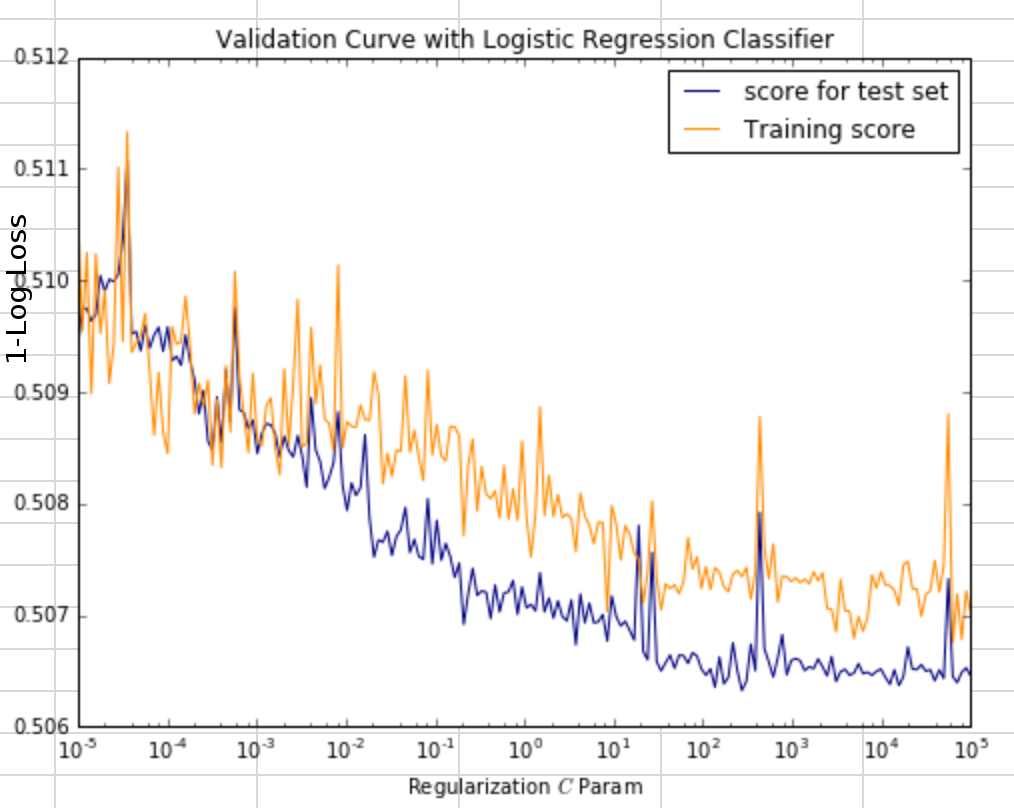
\includegraphics[width=0.9\columnwidth]{figures/regularization/figure-log_loss_error_validation_curve.png}
\caption{ \cref{target1}'s validation curve of a Logistic Classifier model on training and test sets. Here, for each value of the $C$ regularization parameter, we show the score $1 - NLL$. Note that with this formulation, higher scores mean better results.}
\label{fig:log_loss_regularization_validation_curve}
\end{center}
\end{figure}

For the case showed in \cref{fig:log_loss_regularization_validation_curve}, we used all of the features from $\mathcal{T}$ and we generated multiple models $f(x,C)$ where we defined

$$C = \frac{1}{\lambda} $$

In detail, we have that each logistic model was built from a specific $C$ in  $[10^{-5},10^5]$  and the model's negative log loss error ($NLL(C)$) was measured for both $\mathcal{T}$ and $\mathcal{T_s}$ sets separately.
Then, the function of scores $1-NLL(C)$ is graphed as curves over the $C$ value.

As we can see, there is a clear tendency to have better performance across smaller values of $C$ which is equivalent to having stronger regularization of the scoring function.
Note that the $1-NLL(C)$ score will output higher values for better classifiers.
We find that, as a simple case and with no other manipulation of the data, a regularized model helps in having a better performance across the test and training sets error.


\subsection{Hyperparameters}

We can see that in the model built from equation \cref{eq:logitRegularization} there are two specific parameters which we need to predefine before starting the optimization procedure.

Notably we chose the value of $\lambda$ and the ridge regularization method (by selecting the $l2$ penalizing norm over other regularizing functions). %used to measure the size of $\theta$.
It is said these values are \textit{hyper-parameters} of the models since they are not directly part of the theoretical construction yet they need to be previously set in order to find a solution $\theta^\ast$.

In the literature some authors can also refer to the \textit{hyper-parameters} of the model as \textit{tuning parameters}.
These are the values set to configure the different possible variants in the loss function and in the model's training phase.
They will directly affect the estimated fit $f_{\hat{\theta}}$, yet are not the $\theta$ parameter themselves.
They need to be instantiated before training the learner and, as such, they can't be learned from the dataset.

%On the other hand, in a Bayesian context the definition of hyper-parameter is different.
%These appear in the prior distributions of the model's parameters and should not be equated.
%In this case, the parameter's of $\theta$'s distribution are called the hyper-parameters.


%\textit{}

\section{Chapter Summary}\label{section-ch_machine_learning_summary}

We introduced some basic vocabulary on supervised machine learning settings, with references to other types of other non-supervised settings which are not relevant to our general task.
Also, the human mobility problems of this thesis were presented using the aforementioned notation.

A concrete machine learning example was introduced in which we constructed a logistic classifier, where we derivated its loss function from basic theoretical assumptions.
This led us to optimize the hyperplane that best separates the two classes by estimating parameter $\hat{\theta}$.
Given that we now have a problem of $p$ degrees of freedom, we are left to find or fit the parameter $\theta$ by optimizing on certain criteria.
The loss function will then shape our evaluation criteria of saying that one parameter is preferable to another.

Finally, we expanded on the concepts of hyper-parameters and regularization methods which will be reused later in the upcoming sections.


%As we know, a learner will approximate the target with $y \approx \hat{y} = h\left(\sum_{j}\theta_j x^j\right)$.
%
%For example the choice of $0.5$ as a threshold in \cref{formula:logitThreshold} is ad-hoc and certainly one which we could try to fit in the optimization process.
%In the context of machine learning, loss functions give a quantitative measure of a parameter's performance.
%An in binary classification, these are also known as scoring functions.
%the criteria used to choose the best parameters

